\documentclass[../main.tex]{subfiles}
\graphicspath{
    {"../img/"}
    {"img/"}
}
\begin{document}

\begin{przyklad}
    funkcje wielu zmiennych:
\end{przyklad}


\noindent
$\mathbb{R}^{3}\rightarrow\mathbb{R}^{1}$ - Energia potencjalna $\mathcal{V}(x,y,z)$\\
$\mathbb{R}^{4}\rightarrow\mathbb{R}^{1}$ - Potencjał pola niestacjonarnego $\mathcal{V}(x,y,z,t)$\\
$\mathbb{R}^{3}\rightarrow\mathbb{R}^{3}$ - Natężenie pola $\mathcal{E}(x,y,z)$\\
$\mathbb{R}^{4}\rightarrow\mathbb{R}^{3}$\\
$\mathbb{R}^{1}\rightarrow\mathbb{R}^{3}$\\
$\mathbb{R}^{1}\rightarrow\mathbb{R}^{4}$\\
$\mathbb{R}^{1}\rightarrow\mathbb{R}^{6}$\\
$\mathbb{R}^{6}\rightarrow\mathbb{R}^{1}$\\
$\mathbb{R}^{8}\rightarrow\mathbb{R}^{1}$\\

Niech $X\subset\mathbb{R}^n, x_{0} \in X, Y\subset\mathbb{R}^m$. Mówimy, że odwzorowanie $T: X\rightarrow Y$ jest ciągłe, jeżeli $$\underset{x_n \to x_0}{\forall}, T(x_{n})\rightarrow T(x_{0})$$\\
UWAGA: $x_{0} = (x_{1}, x_{2}, ..., x_{n})$.

\vspace{1cm}
\begin{large}
    Pytanie:
\end{large}
Czy ciągłość w $\mathbb{R}^{n} \iff$ ciągłośc w $\mathbb{R}^{1}$?

\begin{przyklad}
    Niech funkcja
\end{przyklad}

\[ f(x,y) =
\begin{cases}
    0                           & \quad x=y\\
    \frac{xy^2}{x^2+y^4}  & \quad x\neq y
\end{cases}
\]

czy $f$ - ciągła w $(0,0)$?
dla trajektorii I:

$$\lim\limits_{y_{n}\to 0}(\lim\limits_{x_{n}\rightarrow 0} f(x_{n},y_{n})) = \lim\limits_{y_{n}\rightarrow 0}(0) = 0$$

dla trajektorii II:

$$\lim\limits_{x_{n}\to 0}(\lim\limits_{y_{n}\rightarrow 0} f(x_{n},y_{n})) = \lim\limits_{x_{n}\rightarrow 0}(0) = 0$$

weźmy $(x_{n},y_{n}) = (\frac{1}{n^{2}},\frac{1}{n})$

$$f(x_{n},y_{n}) = \frac{\frac{1}{n^{2}} \frac{1}{n^{2}}}{\frac{1}{n^{4}}+\frac{1}{n^{4}}} = \frac{1}{2} \neq \lim\limits_{x_{n}\to 0, y_{n}\to 0} f(0,0)$$

\begin{figure}
    \centering
    \begin{center}
        \includegraphics[width=0.48\textwidth]{fig_1}
    \end{center}
    \caption{trajektoria I i II}
\end{figure}

$(X,d_{X})$ - przestrzeń wektorowa z metryką $d_{X},\\ (Y,d_{Y})$ - p.w. z metryką $d_{Y}$

Niech $x_{0}\in X$. Mówimy, że $T: X\to Y$ - ciągłe, jeżeli
$$\underset{\epsilon > 0}{\forall} \quad\underset{\delta}{\exists} \quad\underset{x\in X}{\forall}, \quad d_{X} (x,x_{0}) < \delta \implies d_{Y} (T(x_{0}), T(x)) < \epsilon$$

\begin{dowod}
    Heine $\iff$ Cauchy
\end{dowod}

\begin{large}
    $\implies_{(\text{przez sprzeczność})}$:
\end{large}
\vspace{0.5cm}

zakładamy, że $$\underset{x_n \to x_0}{\forall} T(x_{n}) \to T(x_{0}) \quad\land\quad \underset{\epsilon > 0}{\exists}, \underset{\delta > 0}{\forall}, \underset{x\in X}{\exists} (*): d_{X} (x,x_{0}) < \delta \implies d_{Y} (T(x_{n}),T(x_{0})) \geq \epsilon$$

Skoro $T(x_{n})\to T(x_{0}) \underset{x_n \to x_0}{\forall}$, to w szczególności warunek spełniony dla ciągu, który jest taki:

\vspace{0.3cm}
skoro $(*)$, to dla $\epsilon>0$ weźmy $\delta = 1$,

\begin{align*}
    &\delta=1:\\
    &\underset{x_1}{\exists} \quad d_{X} (x_{1},x_{0})<1 \land d_{Y} (T(x_{1}), T(x_{0})) \geq \epsilon \\
    &\delta=\frac{1}{2}:\\
    &\underset{x_2}{\exists} \quad d_{X} (x_{2},x_{0})<\frac{1}{2} \land d_{Y} (T(x_{2}), T(x_{0})) \geq \epsilon \\
    &\delta=\frac{1}{3}:\\
    &\underset{x_3}{\exists} \quad d_{X} (x_{3},x_{0})<\frac{1}{3} \land d_{Y} (T(x_{3}), T(x_{0})) \geq \epsilon\\
    &\vdots\\
    &\delta=\frac{1}{n}: \underset{x_n}{\exists} \quad d_{X}(x_{n},x_{0}) < \frac{1}{n} \land d_{Y} (T(x_{n}),T(x_{0})) \geq \epsilon
.\end{align*}

Zauważmy, że taki ciąg $x_{n} \to x_{0} \land T(x_{n})\not{\to} T(x_{0})$ i sprzeczność $\Box$

\vspace{0.5cm}
\begin{large}
    $\impliedby$
\end{large}
\vspace{0.5cm}
Wiemy, że $\underset{\varepsilon > 0}{\forall}\quad \underset{x}{\exists}\quad d_{X} (x,x_{0}) < \delta \implies d_{Y} (T(x),T(x_{0})) < \epsilon$ $(\Delta)$, oraz, że $x_{n} \to x_{0}$, czyli:
\[
    \underset{\delta_1}{\forall} \quad\underset{N}{\exists} \quad\underset{n>N}{\forall} \quad d_{X} (x_{n}, x_{0}) < \delta_{1} (\Delta_2)
\]

Chcemy pokazać, że $T(x_n) \to T(x_0)$, czyli, że
$$\underset{\epsilon_1 > 0}{\forall} \underset{N_1}{\exists} \underset{n>N_1}{\forall} \quad d_Y (T(x_n),T(x_0)) < \epsilon_1 (\text{dla } x_n \to x_0)$$

Przyjmijmy $\epsilon=\epsilon_1$. Oznacza to, że $\underset{\delta}{\exists}$ spełniająca warunek $(\Delta)$ dla $\epsilon_1$. Połóżmy $\delta_1=\delta$ we wzorze $(\Delta_2)$, czyli wiemy, że
$$\underset{N}{\exists} \underset{n>N}{\forall} \quad d_X(x_n, x_0) < \delta_1,$$
ale na mocy $(\Delta)$, wiemy, że
$$d_Y (T(x_n),T(x_0)) < \epsilon_1 \Box$$

\subsection{
    Różniczkowalność:
}

Niech $\mathbb{O}\subset\mathbb{R}^{n}, \mathbb{O}$ - otwarty,
$f: \mathbb{O}\to\mathbb{R}^{1}, x\in\mathbb{Q}, x_0 = (x_1^0,x_2^0,\dots,x_n^0)$

Mówimy, że $f$ ma w punkcie $x$ pochodną cząstkową w kierunku $x^k$, jeżeli istnieje granica $g = \lim\limits_{h \to 0}\frac{f(x_1^0, x_2^0, \dots, x_k^0 + h, \dots, x_n^0) - f(x_1^0,\dots,x_n^0)}{h} \equiv \left. \frac{\partial}{\partial x} f \right |_{x=x_0}$

    \begin{przyklad}
        różniczkowalność
    \end{przyklad}

Niech $\mathbb{R}^{2}\to\mathbb{R}^{1}$. $\frac{\partial}{\partial x} f = \lim\limits_{h \to 0}\frac{f(x+h,y) - f(x,y)}{h}, \frac{\partial}{\partial y} f = \lim\limits_{h \to 0}\frac{f(x,y+h) - f(x,y)}{h}$.\\
\vspace{0.3cm}

UWAGA: do policzenia pochodnej czątkowej potrzebujemy układu współrzędnych, tj. (rys)
\vspace{0.3cm}
Niech $\mathbb{O}\subset\mathbb{R}^{n}$, $\mathbb{O}$ - otwarte, $x_0\in\mathbb{O},e\in\mathbb{O},T:\mathbb{O}\to\mathbb{R}$.\\
Mówimy, że $T$ ma w $x_0$ pochodną kierunkową (\textit{spoiler:} pochodną słabą), jeżeli istnieje granica $$g = \lim\limits_{t \to 0}\frac{T(x_0 +te) - T(x_0)}{t} \equiv \nabla_e T(x_0)$$
\subsection{
    Obserwacja:
}
Jeżeli np. $T: \mathbb{R}^{2}\to\mathbb{R}, e_x=(1,0)$ i $e_y = (0,1)$, to $$\nabla_{e_{x}} T = \frac{\partial}{\partial x} T \text{ i } \nabla_{e_{y}} T = \frac{\partial}{\partial y} T$$

\begin{przyklad}

\end{przyklad}
$f(x,y) = \sqrt{|xy|}$. Wówczas $x_0 + te = (0+t1,0)$, $x_0 = (0,0), e_x = \binom{1}{0}$

$$\left. \nabla_{e_x} f \right |_x=(0,0) = \lim\limits_{t \to 0}\frac{f(0+t,0) - f(0,0)}{t} = \lim\limits_{t \to 0}\frac{\sqrt{|t 0|} - \sqrt{|0 0|}}{t} = \lim\limits_{t \to 0}\frac{0}{t} = 0 = \left. \frac{\partial}{\partial x} f\right |_{(0,0)}$$

UWAGA: $f(x) = \sqrt{x}, \mathbb{R}\to\mathbb{R}, f'(0) = \lim\limits_{h \to 0}\frac{\sqrt{h}}{h} = \pm \infty$

\[ f(x,y) =
\begin{cases}
    0 & \quad x=y\\
    \frac{xy^2}{x^2+y^4} & \quad x \neq y\\
\end{cases}
\]

$e = \binom{h_1}{h_2}$. Pochodna: $\left. \nabla_e f\right |_{x=(0,0)}, (x_0 + te = (th_1, th_2))$

$$\lim\limits_{t \to 0}\frac{f(th_1, th_2) - f(0,0)}{t} = \frac{h_1 h_2^2}{h_1^2} = \frac{h_2^2}{h_1}$$

\begin{figure}
    \centering
    \includegraphics[width=0.8\textwidth]{fig_2}
    \caption{Problemy: Umiemy tak jak po lewej, ale nic nie potrafimy zrobić z tym po prawej}
    \label{fig:fig_2}
\end{figure}

\end{document}
